% Integrated from research_report/member_4/zhitong_sections.tex.
\subsection{Uncertainty and Accent Variation}
\label{sec:statistical-results}

Paired comparisons assess whether the quality ranking is supported after
accounting for speaker dependence. Separate analyses examine the spread of
accent means and whether the size of each system gap varies across accents.

\begin{table}[t]
\caption{Paired mean sentence chrF++ gaps (points) with speaker-clustered 95\% intervals. Positive gaps favour the first-named system.}
\label{tab:paired-gaps}
\centering
\small
\begin{tabular}{lcc}
\toprule
Comparison & Mean gap & 95\% CI \\
\midrule
Direct $-$ Cascade-600M & $+7.00$ & [6.45, 7.60] \\
Direct $-$ Cascade-3.3B & $+4.99$ & [4.39, 5.70] \\
Cascade-3.3B $-$ Cascade-600M & $+2.01$ & [1.61, 2.42] \\
\bottomrule
\end{tabular}
\end{table}

\begin{table}[t]
\caption{Mean sentence chrF++ by accent and Direct-minus-Cascade gaps with speaker-clustered 95\% intervals (unadjusted for multiplicity). Eng, Fil, HK, Ind, Mal, SAf, US = England, Filipino, Hong Kong, India and South Asia, Malaysian, Southern African, United States; $n_{\mathrm{spk}}$ = speakers; D, C6, C3 = Direct, Cascade-600M, Cascade-3.3B.}
\label{tab:accent-gaps}
\centering
\footnotesize
\setlength{\tabcolsep}{3pt}
\begin{tabular}{lrcccrr}
\toprule
Accent & $n_{\mathrm{spk}}$ & D & C6 & C3 & D$-$C6 & D$-$C3 \\
\midrule
Eng & 398 & 27.9 & 22.5 & 23.6 & 5.4 [4.3, 6.5] & 4.2 [3.1, 5.3] \\
Fil & 72 & 28.9 & 21.2 & 24.5 & 7.7 [6.2, 9.3] & 4.4 [3.2, 5.8] \\
HK & 41 & 28.3 & 20.0 & 21.3 & 8.4 [6.1, 10.2] & 7.0 [4.6, 9.7] \\
Ind & 356 & 27.4 & 19.8 & 22.0 & 7.6 [6.5, 8.9] & 5.4 [4.3, 6.7] \\
Mal & 61 & 28.0 & 20.2 & 22.4 & 7.9 [6.5, 9.3] & 5.7 [4.5, 7.0] \\
SAf & 131 & 27.2 & 21.7 & 23.7 & 5.5 [4.3, 6.7] & 3.5 [2.5, 4.6] \\
US & 527 & 27.3 & 20.7 & 22.6 & 6.6 [5.4, 7.8] & 4.7 [3.6, 5.8] \\
\bottomrule
\end{tabular}
\end{table}

\subsubsection{System gaps}
All three overall gap intervals exclude zero (Table~\ref{tab:paired-gaps}),
supporting Hypotheses~\ref{hyp:quality} and~\ref{hyp:mt-size}.
Cascade-3.3B gains about two points over Cascade-600M.
Within every accent the
Direct-minus-Cascade intervals also exclude zero (Table~\ref{tab:accent-gaps}),
and the speaker-level matched-pairs rank-biserial correlations are positive
throughout (0.53--0.93 against Cascade-600M; 0.39--0.91 against Cascade-3.3B).

The Cascade-3.3B lift is positive in all seven accents. Its mean-gap bootstrap
intervals remain above zero for England English (0.18 to 2.19) and Hong Kong
English (0.09 to 2.52), whereas the speaker-level Wilcoxon tests give
$p=0.138$ and $0.089$. These procedures assess different quantities: the
bootstrap estimates the clip-weighted mean gap, while the rank test uses
speaker-mean paired differences. The two summaries therefore need not agree.

\subsubsection{Accent means and spread}
\begin{figure}[t]
\centering
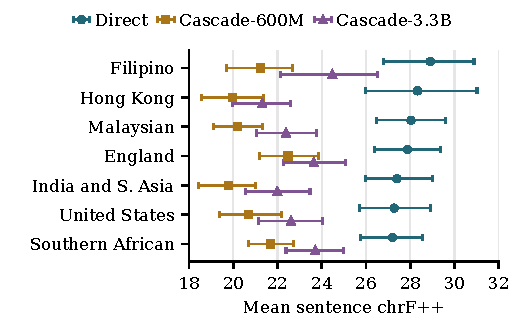
\includegraphics[width=\columnwidth]{figures/accent_means.pdf}
\caption{Mean sentence chrF++ with unadjusted 95\% speaker-clustered
bootstrap intervals. Overlap alone does not test robustness differences.}
\label{fig:accent-means}
\end{figure}

Direct has the smallest observed between-accent spread, but the differences
between systems remain uncertain (Fig.~\ref{fig:accent-means}).
The spread $R_s$ is 1.71 [1.4, 5.1] points
for Direct, 2.70 [2.0, 4.7] for Cascade-600M and 3.17 [2.0, 5.7] for
Cascade-3.3B. These intervals are right-skewed because a maximum minus a minimum
of noisy means is biased upward. All three differences in spread have
intervals that include zero (e.g.\ $-1.0$ [$-2.3$, 2.3] for
Direct $-$ Cascade-600M). Higher translation scores therefore do not establish
stronger accent robustness under the study's spread-based definition;
Hypothesis~\ref{hyp:spread} remains unresolved.

A speaker-level Kruskal--Wallis test detects accent differences only for
Cascade-600M ($p=0.041$, $\epsilon^2=0.008$; Direct $p=0.185$,
Cascade-3.3B $p=0.168$), a single uncorrected result. The cascades largely agree
in their accent orderings (Spearman $\rho=0.82$), whereas Direct follows neither
($\rho=-0.18$ and $-0.07$; seven means only). Hong Kong English ranks second
for Direct but sixth or seventh for the cascades, and its intervals are wide
because it has only 41 speakers.

\subsubsection{Variation in system gaps across accents}
\label{sec:statistical-accent-gap-variation}
The Direct-minus-Cascade gap varies across accents, with small speaker-level
effects against Cascade-600M ($H(6)=21.4$, $p=0.0015$, $\epsilon^2=0.014$)
and Cascade-3.3B ($H(6)=17.2$, $p=0.009$, $\epsilon^2=0.011$); clip-level
tests agree. Against Cascade-600M the gap is largest for Hong Kong English
(8.4) and smallest for England English (5.4); against Cascade-3.3B it is
largest for Hong Kong English (7.0) and smallest for Southern African
speakers (3.5).

Few individual accent pairs differ after correction: 2 of 21 against
Cascade-600M and 1 of 21 against Cascade-3.3B, all with small effects
(Cliff's $|\delta|\le 0.30$). Malaysian versus United States English is the
pair common to both. Clip-level tests flag different pairs, so pair-level
conclusions are fragile. Direct's flatter accent means suggest that the
variation comes mostly from the cascades, but the uncertain spread differences
prevent a firm conclusion. The Cascade-3.3B lift shows no detectable variation
across accents ($p=0.168$ speaker level); this does not establish equal gains.

\subsection{Recognition Errors and Translation Scores}
\label{sec:statistical-asr-associations}
The accent-level WER pattern in Table~\ref{tab:accent} motivates a clip-level
analysis of recognition and translation scores. Higher normalized WER is
associated with lower cascade scores ($\rho=-0.19$ [$-0.22$, $-0.16$] for
Cascade-600M; $-0.20$ [$-0.23$, $-0.17$] for Cascade-3.3B) and with a larger
Direct advantage ($\rho=0.13$ [0.10, 0.16] and $0.17$ [0.14, 0.20]). All
intervals exclude zero, overall and within each accent, supporting
Hypothesis~\ref{hyp:wer}. The associations are weak and observational;
they do not identify ASR error as the cause.

These associations describe the cascade's exposed recognition stage. The
following diagnostics examine a separate feature of Direct outputs: the
visible \unk{} marker. Section~\ref{sec:synthesis-results} then compares
system gaps within WER-defined subsets.
